\begin{figure}
\begin{fullpage}
        \begin{center}
        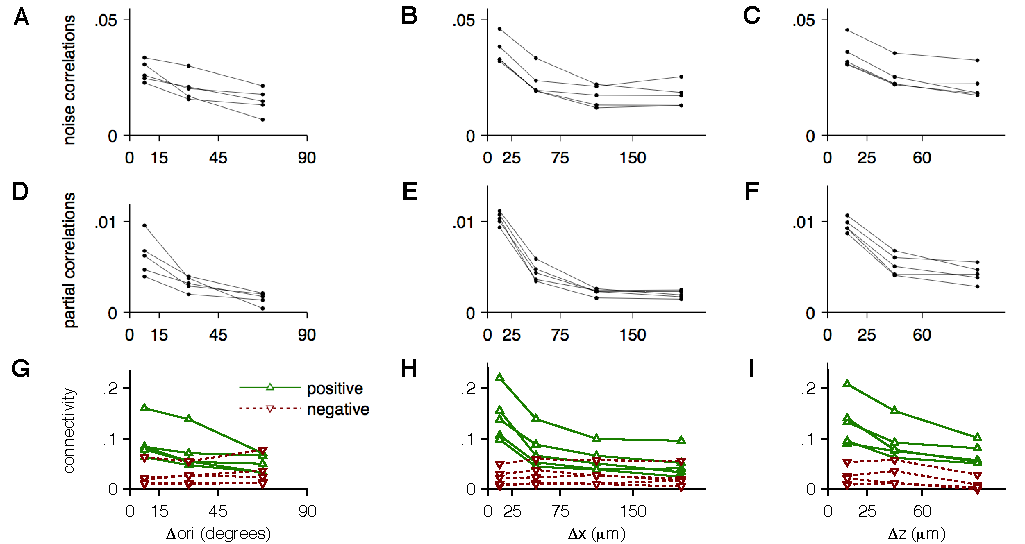
\includegraphics[width=\textwidth]{./figures/Figure7.pdf}
        \end{center}
        
\caption[Relationship between functional connectivity and circuit architecture]{
{\bf Relationship between functional connectivity and circuit architecture}
Dependence of sample correlations, regularized partial correlations, and connectivity inferred by $C_{\sf sparse+latent}$ on the differences in preferred orientations, $\Delta \mbox{ori}$, and physical distances: horizontal $\Delta x$ and depth $\Delta z$.
Five sites with highest connectivity (see Fig.~\ref{fig:6} B) were selected for this analysis.
\\
{\bf A--C.} Mean sample correlations in relation to $\Delta\mbox{ori}$,  $\Delta x$ and $\Delta z$, respectively. For $\Delta x$ averages, only horizontally aligned cell pairs with $\Delta z<30\,\mu m$ were considered. Similarly, for $\Delta z$ averages, only vertically aligned cell pairs with $\Delta x<30\,\mu m$ were considered.
\\
{\bf D--F.} Mean partial correlations regularized by the $C_{\sf sparse+latent}$ estimator binned the same way as the sample correlations above. The partial correlations exhibit stronger dependence on $\Delta\mbox{ori}$, $\Delta x$, and $\Delta z$ than sample correlations. 
\\
{\bf G--I.} Positive connectivity (green) and negative connectivity (red) inferred by the $C_{\sf sparse+latent}$ estimator. 
Positive and negative connectivities refer to the fractions of the positive and negative partial correlations computed from the sparse component $S$ of $C_{\sf sparse+latent}$.  
Positive connectivity decreases with $\Delta \mbox{ori}$, $\Delta x$, and $\Delta z$. 
Negative connectivity does not decrease with $\Delta \mbox{ori}$, $\Delta x$ within the examined range, and with $\Delta z$ for small values of $\Delta z<60\,\mu m$.
}\label{fig:7}

\end{fullpage}
\end{figure}
